\documentclass[10pt]{jreport}
\usepackage{geometry}
\geometry{left=15mm,right=15mm,top=20mm,bottom=20mm}
\usepackage[dvipdfmx]{graphicx}
\renewcommand\thefootnote{\arabic{footnote})}
\begin{document}
{\LARGE Debugging Usually Slightly Broken (USB) Devices and Drivers}\\\\
USBに関する高度なデバッグについてのプレゼン.USB Deviceのマネジメント,USB Driverの修正についての話.

\begin{description}
  \item {\large \textbf{1. USB basics}}\mbox{}\\
  USBはデータのやり取りができるバスで,ストレージやプリンタなど様々なレベルのサービスを提供できる.\\
  →USB DeviceはUSB Host(PCなど)に対して機能を提供する.USB Hostは同時に様々なUSB Deviceと接続できるが,USB Deviceは同時に複数のUSB Hostと接続はできない.
  1つのUSB Deviceは最大31個のEndpoint
  \footnote[1]{Endpoint:USB DeviceとHostがデータのやり取りするためのFIFOバッファ}
  を保持している
  \begin{itemize}
    \item Endpoint 0はどのDeviceでも必ず使う.Host←→Deviceの通信ができる(コントロール転送)
    \item 他には,IN と OUTがあり,IN はDevice→Host,OUT はHost→Deviceの通信ができる
    \item IN,OUT それぞれ15個の割り当てがされ,1 + 15 + 15 = 31個
    \end{itemize}\\
    Endpointには4種類の転送方法がある
    \begin{itemize}
      \item Control転送:     双方向転送可能でEndpoint0が使える.アプリケーションに利用可能
      \item Bulk転送:        画像などの大きいデータや時間に依存しないデータの転送に使われる
      \item Interrupt転送:   待ち時間が短いようなデータや時間に依存するデータの転送に使われる
      \item Isochronous転送: サイズが大きく時間に依存するデータの転送に使われる
      \end{itemize}\\
      \begin{center}
        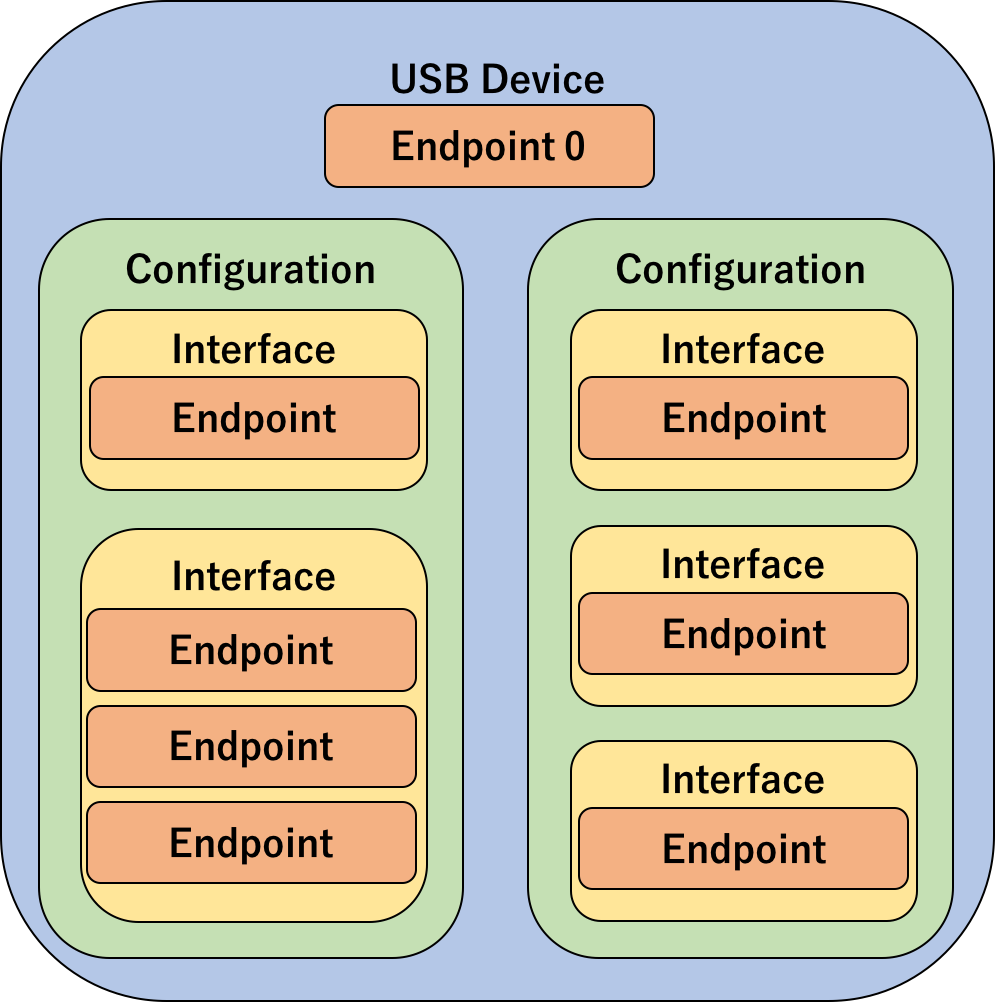
\includegraphics[width=5cm]{img/USB-1.png} \\
        Figure1: USB Device, Configuration, Interface and Endpoint
      \end{center}
      EndpointはInterfaceの中でグループ化され,InterfaceはConfigurationの中でグループ化される.USBデバイスは複数のConfigurationを持つ.Interfaceは機能の提供,Configurationは設定の提供.ConfigurationとInterfaceはそれぞれ1つずつしか動作させられないので,あるEndpointを利用できないタイミングがある.Endpoint 0はグループ化されないので,いつでも利用できる.\\\\
      このほかにUSB Descriptor
      \footnote[2]{接続されたUSB Deviceはどのような機器なのかをHostが把握するためのデータ}
      という重要な要素がある.
      \begin{itemize}
        \item Device Descriptor: Device Driverを選ぶための製品IDや企業IDなどの情報
        \item Configuration Descriptor: Deviceの構成情報 必要な電力
        \item Interface Descriptor: Deviceの機能を表す情報
        \item Endpoint Descriptor: Endpointの転送種類や方向などの情報
      \end{itemize}
      USBと接続するためには,Device Driverで接続,転送する機能を作成する必要がある.しかし,特定機能(Device Class)は作成する必要がない.
      \begin{center}
        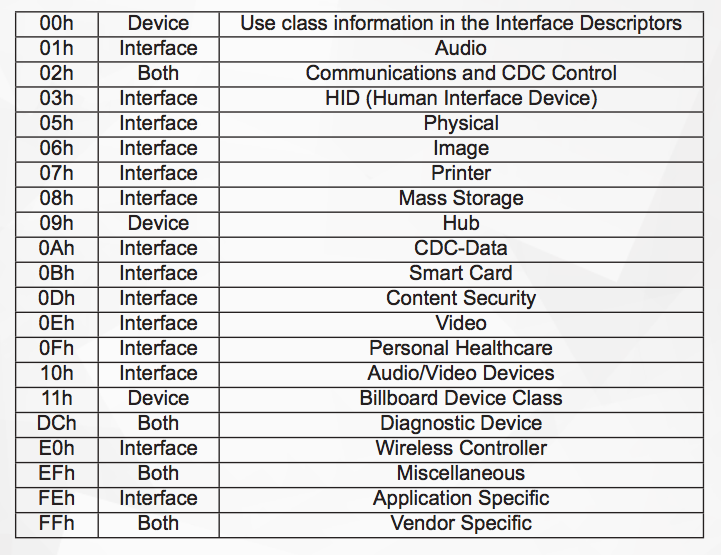
\includegraphics[width=5cm]{img/USB-2.png} \\
        Figure2: USB Classes
        \end{center}\\\\

        \item {\large \textbf{2. Plug \& Play}}\mbox{}\\
        USB Deviceを接続してから利用できるまで何が起きているか.
        \begin{enumerate}
          \item Deviceを接続する
          \item Hostは接続を検知する
          \item アドレスをセットする
          \begin{enumerate}
            \item 128個のアドレスを持つことができ,デフォルトは0x00.Deviceごとに++したアドレスを割り当てる
          \end{enumerate}
          \item Deviceの情報(Descriptors)を入手する
          \item Configurationを選択する
          \begin{enumerate}
            \item Configurationが一つだけなら問題はない
            \item 複数ある場合は,選択したConfigurationのInterfaceを利用できるのでそれを利用する
          \end{enumerate}
          \item InterfaceのためのDriverを選択する (Deviceではなく"Interface"のための選択)
          \begin{enumerate}
            \item カーネルコードの一部(モジュール)のstruct usb\_driverを使う
            \begin{enumerate}
              \item struct usb\_driverはuser spaceにnetwork interfaceやblock deviceなどを提供する
              \item いくつかの通信プロトコルによって実装され,web browserやssh clientに似ている
            \end{enumerate}
            \item 登録したDriverのリストをカーネルは保持しており,Driverには対応しているDevice IDが記されている
            \item このDriverリストにあるDevice IDとDevice Descriptorを比較して一致したDriverを選択する
          \end{enumerate}
          \item USB Deviceが使えるようになる
          \end{enumerate}\\\\

          \item {\large \textbf{3. Plug \& do what I want}}\mbox\\
          すべて自動で処理ことは良いが,いつでも自動で処理されるのはよろしくない.USBに関することがすべて自動で処理されるとセキュアなシステムとは言えない.
          \begin{itemize}
            \item 一部のデバイス機能だけが必要だが,多くのデバイスを許可してしまう
            \item 間違ったConfigurationやDriverを選択する可能性がある
          \end{itemize}
          USBのシステム構成は3種類存在する
          \begin{itemize}
            \item usbX : Hostのポートに接続しているもの
            \item X-A.B.C : 1つのハブのポートに接続しているもの
            \item X-A.B.C:Y.Z : 1つのハブにハブ2を繋げ,ハブ2のポートに接続しているもの
          \end{itemize}
          許可するDevice数の上限を設定する
          \begin{itemize}
            \item USB Deviceはauthorizedという属性を持つ
            \item usbXはauthorized\_defaultという属性を持つ
            \item authorizedが0であれば,Deviceは未構成で,承認された時にusbguardがDriverの選択を自動で行う
          \end{itemize}
          Linuxカーネルv4.4からは,これが改善された
          \begin{itemize}
            \item USB Interfaceがauthorized属性を持つ→Configurationを選択できる
            \item usbXはinterface\_authorized\_default属性を持つ
            \item autorizedが0であれば,Driverはバインドされず,Driverの選択をする際は手動で行う
          \end{itemize}
          カーネルが選択するConfigurationを変更することができる
          \begin{itemize}
            \item USB Deviceが持つbConfigurationValueを変更すると良い
          \end{itemize}
          Device IDをDriverに追加することができる
          \begin{itemize}
            \item 多くのDriverはVendor IDとProduct IDがペアになっている
            \item しかし,ベンダーによってはDriverからこのペアを削除したり,VIDが間違っていたりする
            \item これらを改善するためには,DriverのDevice ID Tableを変更する必要がある.
          \end{itemize}
          IDは動的に変更させることができ,その形式は3通りある.ただし,それぞれ16進数で書かないといけない
          \begin{itemize}
            \item VID+PID
            \item VID+PID+Intf Class
            \item VID+PID+Intf Class+dev_info:
            \begin{itemize}
              \item \$RefVIDと\$RefPIDはデバイステーブルへの登録をするもの
            \end{itemize}
          \end{itemize}
          新しいDeviceIDをDriverに追加したいときはDriverが持つnew\_idファイルに書き込めば良い\\
          DeviceIDを消したいときは,Driverが持つremove\_idファイルに書き込めば良い\\
          特定のInterfaceをバインドしたいときはbindファイル,解除したいときはbindファイルに書き込めば良い\\\\

          \item {\large \textbf{4. Plug \& tell me more}}\mbox\\
          ここまで紹介してきた方法だと,予期せぬ問題や振る舞いが起きてしまい,コードをデバッグしようとしても何が問題かわからない\\
          USBはホストを制御するバスで,Deviceを使うにはホストはUSBを初期化しないといけない.USBはポーリング
          \footnote[3]{ポーリング:連携動作する際に、送信/処理要求がないか、一つ一つの相手に確認する方式}
          されたバスで,ホストはそれぞれのDevieをポーリングしてデータの要求や送信をする.\\
          USB transportの話をするとTranferの中にtransactionが存在する.
          \begin{itemize}
            \item transactionでは,Endpointに指定されたパケット上限までのデータを渡す
            \item transferは,複数のtransactionを持ち,そのtransactionの長さは可変である
            \item transactionはHost Controller DriverやUSB Device Driverの操作であるため,かなり低いレイヤーである
          \end{itemize}
          Linuxカーネルでは,transferはUSB Request Block(URB)\footnote[4]{USBバスを通って送られてきたデータのまとまり}になっている\\
          典型的なUSB DriverはUSBに関わる3つの関数とユーザ空間で使うような関数から成り立っている
          \begin{itemize}
            \item probe()      : Deviceをチェックしてリソースを割り当て
            \item disconnect() : リソースを解放する
            \item complete()   : 状態を確認して,データを朱徳したり,再送信したりする
          \end{itemize}
          USB Deviceでの典型的なバグ
          \begin{itemize}
            \item Descriptorが間違っていること
            \item 何かミスがあった時のエラーパスがないこと
            \item complete()での正しいエラー処理がないこと
            \item パケットの形式が正しくないこと
          \end{itemize}
          HW USB sniffersというUSB Driverの性能やプロトコルの性能を評価することができるツールがある.かなり便利であるが高額.Open Hardwareなら材料費約100\$で作ることができる.\\
          USB monitorは,sumit()やcomplete()などのUSBに関わるイベントのログを取るのだが,transferレベルのデータしか取れないず,transactionレベルのデータを取得できない.\\
          URBバッファのデータは常に妥当であるわけではない.妥当性はtransferの結果とEndpointの方向方向によって決まる.
          \item {\large \textbf{5. Summary}}\mbox\\
          \begin{itemize}
            \item USB Descriptorはポートのようなもの
            \item lsusbを使うことで情報を取得できる
            \item 各Device Driverは互換性のあるDeviceリストを宣言する
            \item USB DeviceはSysFSを通して管理することができる
            \item DriverはURBを用いて通信する
            \item Open HardWareを使えば,USB trafficを監視するのに膨大な金額を使う必要はない
          \end{itemize}
          \end{document}
